\section{Water in the Climate System}
\label{sec:water_in_climate}

Figure \ref{fig:soden_held} shows us the radiative feedback of various parameters (see section \ref{sec:forcing_feedback}).
In this section we will focus on how these parameters lead to a positive or negative radiative feedback.

\begin{figure}[h]
    \centering
    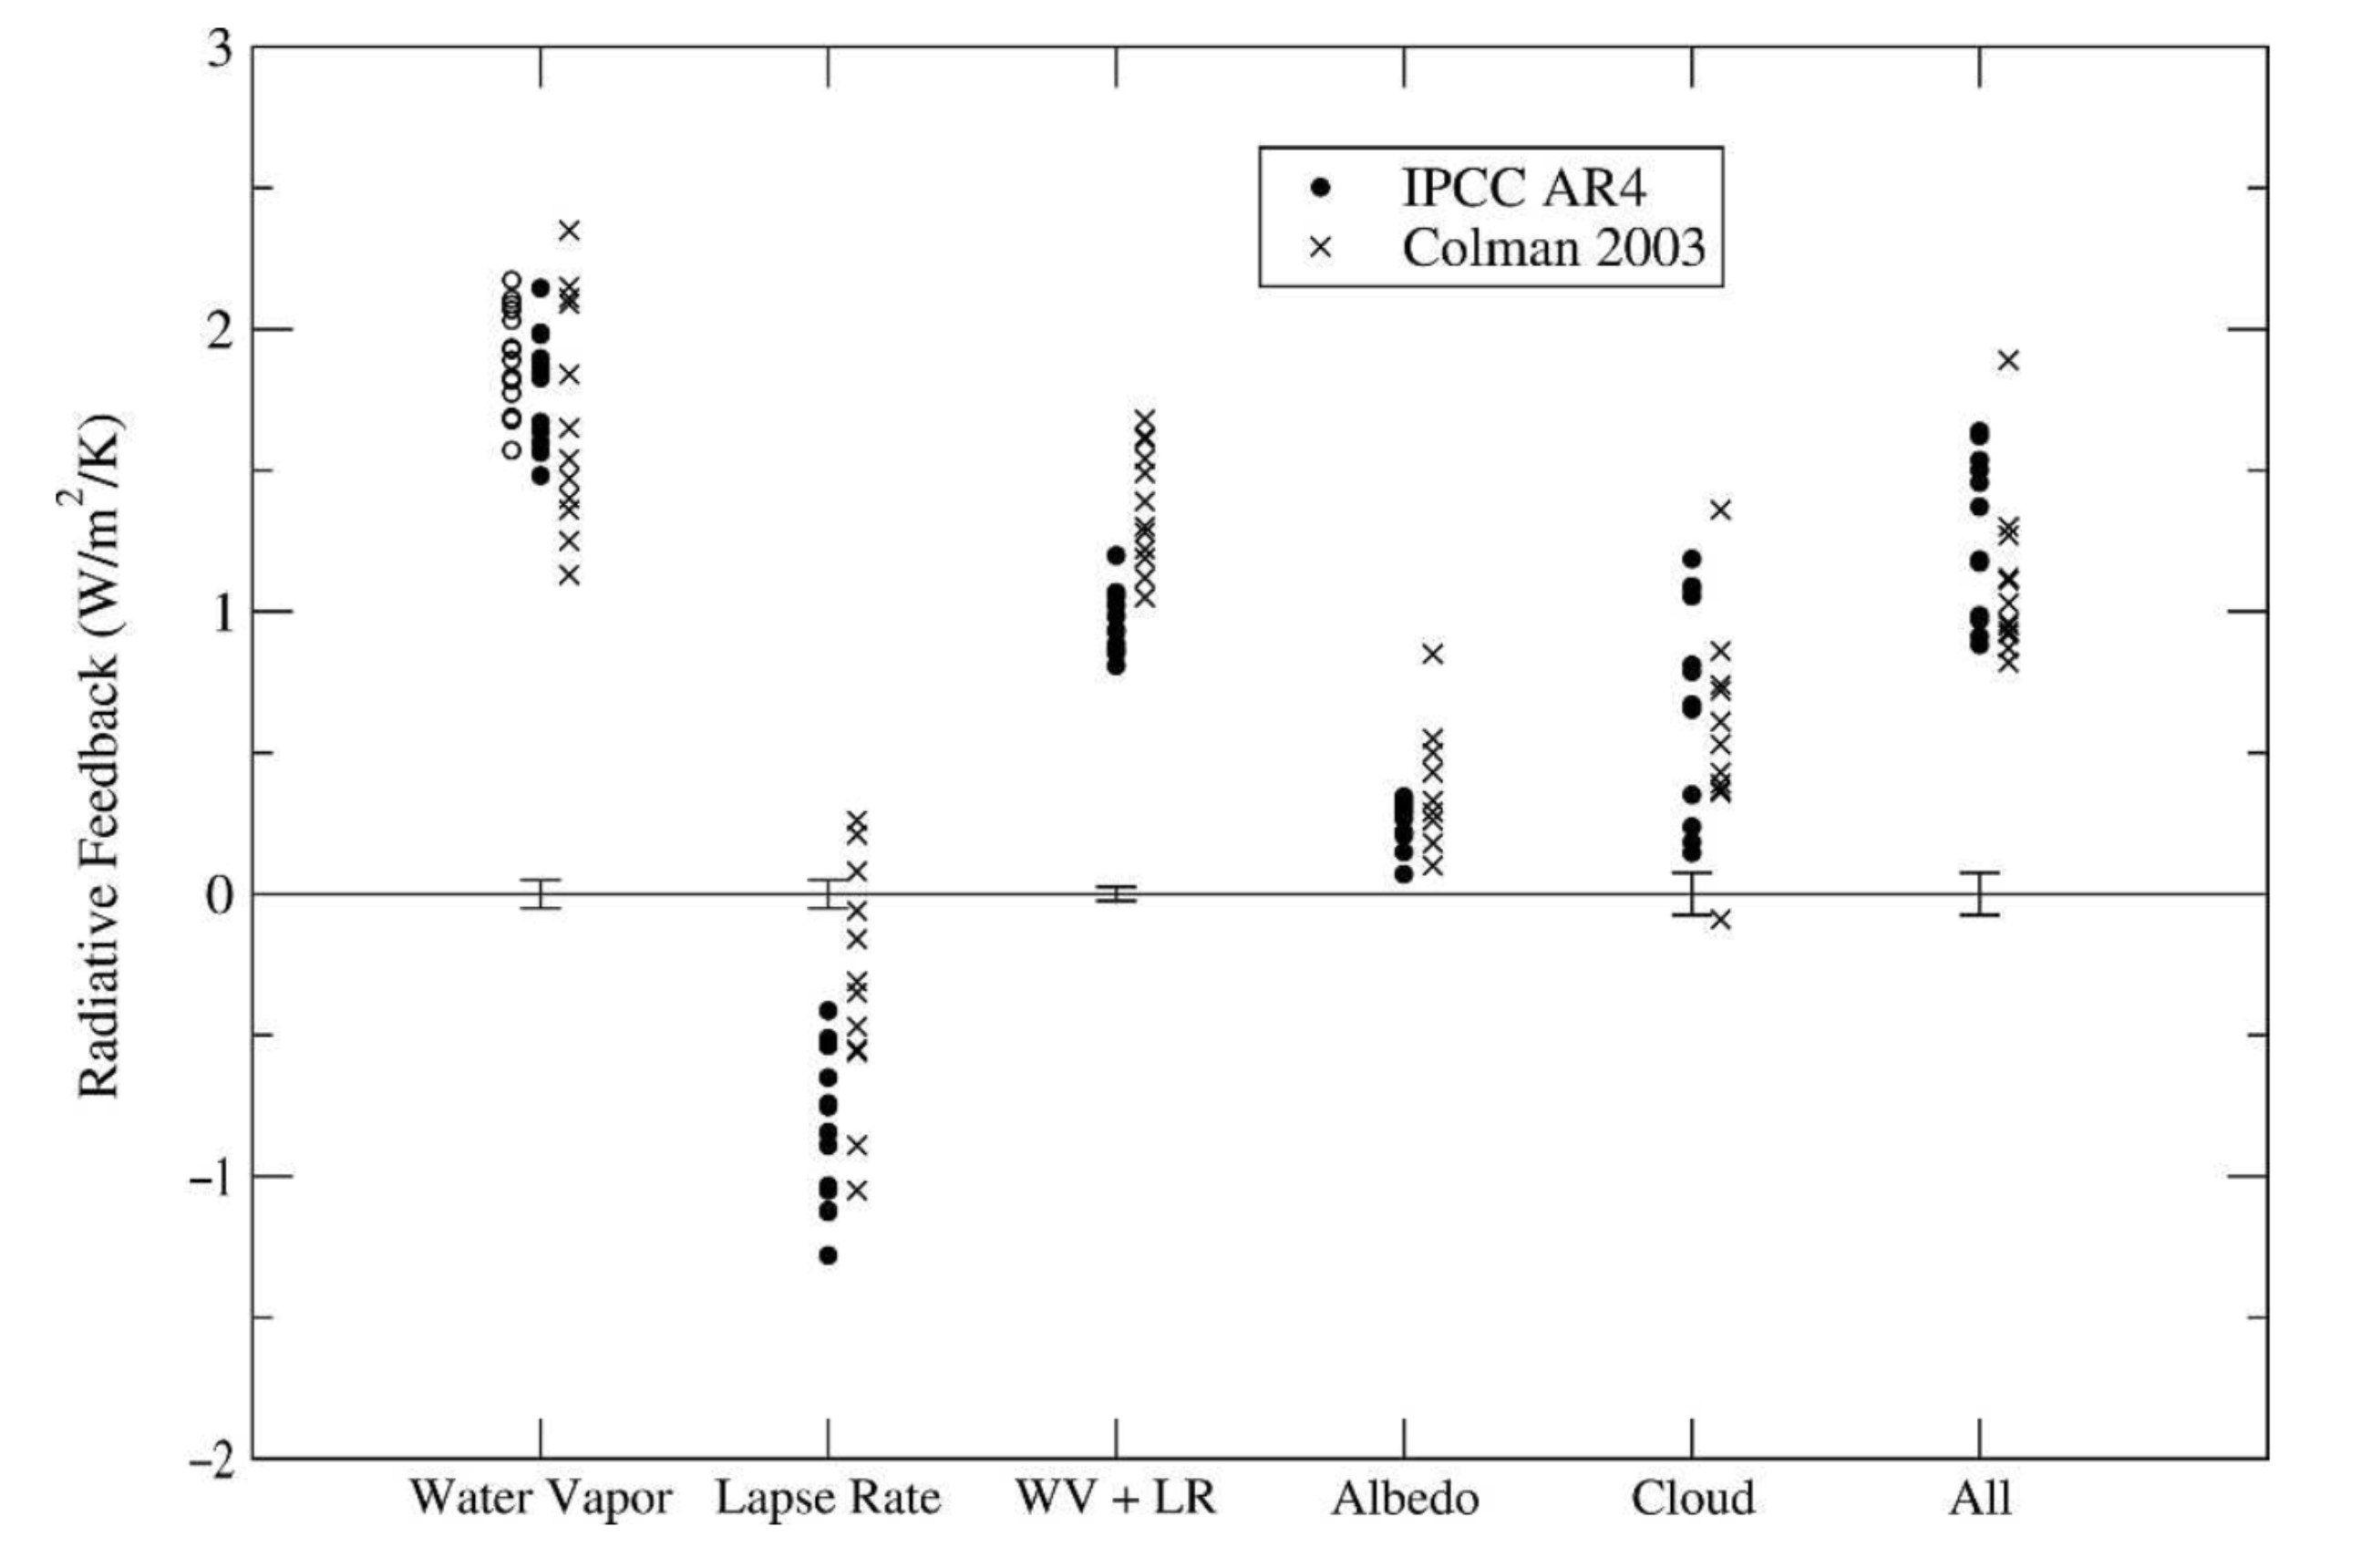
\includegraphics[width=0.75\textwidth]{figures/Soden and Held 2006.png}
    \caption{Radiative Feedback of Various Parameters (\cite[Soden and Held 2006]{soden_held_2006}).}
    \label{fig:soden_held}
\end{figure}

\subsection{Ice-Albedo Feedback}
\label{sec:ice_albedo_feedback}

The distribution of sea-ice shows a natural seasonability linked to the pattern of solar radiation at the surface with a
maximum etent at both poles after their respecive polar nights (and vice versa). Over the last few decades, satellite
observations have shown a clear decrease in the extent of sea-ice in the arctic (this is not the case in the Antarctic,
where the pattern seen is different. There is no clear sign of decreasing of sea-ice, in fact there are signs of a slight
increase. The reasons why are still up for debate and more recent data post 2017 show a decrease as expected with the
warming of the climate. This is non-examinable).

The \textbf{ice-albedo feedback} mechanism suggests that an increase in surface temperature would result in a reduced 
snow and sea-ice cover and hence reduce \hyperlink{albedo}{surface albedo} ($\alpha$). This would result in a decrease in
planetery albedo $\alpha_p$ and hence an increase in absorbed solar radiation. This would lead to a further increase in
surface temperature and so on. This is a \textbf{positive feedback} mechanism as shown in Figure \ref{fig:soden_held}.

\subsection{Lapse Rate}
\label{sec:lapse_rate}

The \textbf{lapse rate} is the negative rate at which temperature changes with height in the atmosphere. In the troposphere,
where the temperature decreases with height, the lapse rate is positive. We define lapse rate $\Gamma$ as:
$$
\Gamma = -\frac{dT}{dz}
$$
where $T$ is temperature and $z$ is height.

For a parcel of dry air lifted in an atmosphere due to convection, it follows that it does so adiabatically. In this case
we say that it rises at the \textbf{dry adiabatic lapse rate} $\Gamma_d$. 
$$
c_PdT - vdP = dq \quad \text{1st Law of Thermodynamics} \\
$$
$$
\frac{dT}{dz} = - \frac{g}{c_P} \quad \implies \quad \boxed{\Gamma_d = \frac{g}{c_P}}
$$

The same thing happens for a parcel of moist air. We begin by imagining a parcel 
of air near the surface that contains some non-zero amount of water vapour. As the
parcel rises, it cools adiabatically so it gets closer and closer to its saturation
point. Eventually it does, and the height at which it reaches the saturation point
is called the \textbf{lifting condensation level (LCL)}. At this point, the parcel
condenses and releases latent heat as it rises further. This heat means the parcel's
temperature does not decrease as fast as it otherwise would. Such a parcel is said
to be following the \textbf{moist adiabatic lapse rate} $\Gamma_s$.

% Make z-T diagram showing dry and moist adiabatic lapse rates showing the difference in slopes and the LCL
\begin{figure}
    \centering
    \begin{tikzpicture}
        \begin{axis}[
            xlabel=$T$,
            ylabel=$z$,
            xmin=0, xmax=10,
            ymin=0, ymax=10,
            % xtick={},
            % ytick={},
            yticklabels={},
            xticklabels={},
            axis lines=middle,
            axis line style={-},
            width=0.7\textwidth,
            height=0.7\textwidth,
            grid=major,
            grid style={dashed, gray!30},
            % legend pos=north east,
            % legend style={font=\small, cells={align=left}},
            % legend cell align={left},
        ]
        \addplot[domain=1:5, samples=100, color=blue]{-1.5*x + 10}
        node[pos=0, above]{$\Gamma_s$};

        \addplot[domain=1:9, samples=100, color=red]{-0.5*x + 5}
        node[pos=0, above]{$\Gamma_d$};

        \addplot[dotted, thick, domain=2:8, samples=100, color=black]{2.5}
        node[pos=0.5, above right]{$LCL$};
        \end{axis}
    \end{tikzpicture}
    \caption{Dry and Moist Adiabatic Lapse Rates.}
    \label{fig:adiabatic_lapse_rates}
\end{figure}

We can combine the two lapse rates into one equation as follows (see handout 2, moist adiabatic lapse rate for derivation):
$$
\Gamma_s = \Gamma_d \frac{1 + \frac{w_s l_v}{R_d T}}{1 + \frac{\epsilon l_v^2 w_s}{c_p R_d T^2}} = \Gamma_d \frac{1+X}{1+bX}
$$
where $l_v$ is the latent heat of vapourisation, $w_s$ is the \textbf{saturation mixing ration}, $T$ is the temperature,
$R_d$ is the gas constant for dry air, $c_p$ is the specific heat capacity of dry air at constant pressure, $\epsilon$ is
the ratio of the gas constants for dry air and water vapour, $X = \frac{w_sl_v}{R_dT}$ and $b = \frac{\epsilon l_v}{c_pT}$.

To summarise, and worth noting is the following:
$$
\boxed{\Gamma_d = \frac{g}{c_p}\ , \quad b > 1 \ , \quad \Gamma_s < \Gamma_d}
$$

\subsection{Lapse Rate Feedback}
\label{sec:lapse_rate_feedback}

We showed in section \ref{sec:lapse_rate} that the rate of change of $\Gamma_s$ with temperature must be negative. In 
regions of high moisture and convective uplift (e.g. tropical troposphere) a change in surface temperature will in turn
lead to a change in the atmosperic temperature at higher altitudes. If we have a radiative \hyperlink{glo:forcing}{forcing}
which results in a surface warming, this will lead to a decrease in $\Gamma_s$ (the gaph in Figure \ref{fig:lapse_rate_feedback}
gets steeper). In other words the temperature at higher altitudes will increase more than ``expected'', the graph does
not simply translate. We can see this in Figure \ref{fig:lapse_rate_feedback}.

\begin{figure}
    \centering
    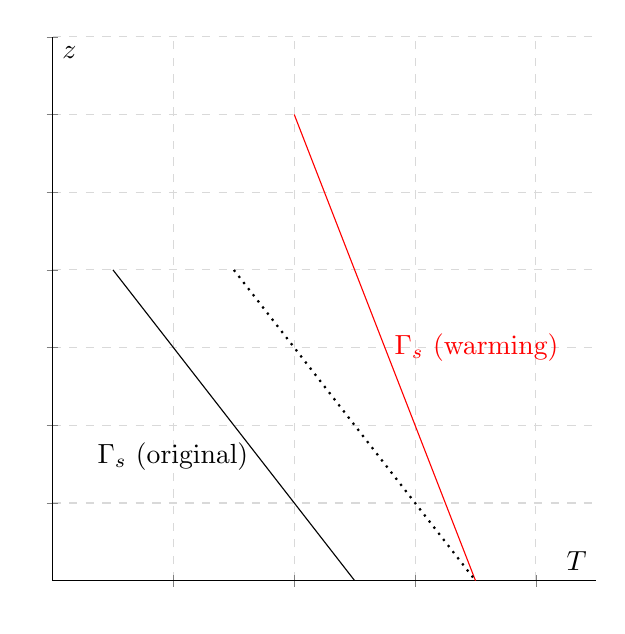
\begin{tikzpicture}
        \begin{axis}[
            xlabel=$T$,
            ylabel=$z$,
            xmin=0, xmax=9,
            ymin=0, ymax=7,
            % xtick={},
            % ytick={},
            yticklabels={},
            xticklabels={},
            axis lines=middle,
            axis line style={-},
            width=0.7\textwidth,
            height=0.7\textwidth,
            grid=major,
            grid style={dashed, gray!30},
            % legend pos=north east,
            % legend style={font=\small, cells={align=left}},
            % legend cell align={left},
        ]
        \addplot[domain=4:7, samples=100, color=red]{-2*(x - 2) + 10}
        node[pos=0.5, right]{$\Gamma_s$ (warming)};

        \addplot[domain=1:9, samples=100, color=black]{-x + 5}
        node[pos=0.3, left]{$\Gamma_s$ (original)};

        \addplot[dotted, thick, domain=3:7, samples=100, color=black]{-x + 7};
        % node[pos=0, above]{$\Gamma_s$};

        \end{axis}
    \end{tikzpicture}
    \caption{Lapse Rate Feedback.}
    \label{fig:lapse_rate_feedback}
\end{figure}

Figure \ref{fig:lapse_rate_feedback} shows that the lapse rate feedback is negative. This means that a radiative forcing
will lead to a greater change in temperature at higher altitudes than expected. This is a positive feedback because
the change in temperature at higher altitudes will lead to a greater \gls{LW} emission at the \gls{TOA} (equivalently,
an increase in \gls{OLR}) and also a net decrease in \gls{LW} emission back towards the surface. This will therefore 
lead to a cooling of the surface, hence negative feedback.

\subsection{Lapse Rate and Water Vapour Feedback Combined}
\label{sec:lapse_rate_water_vapour_feedback}

We have seen in section \ref{sec:clausius-clapeyron} that relative humitidy tends to be conserved i.e. if atmospheric
temperature increases or decreases, the relative humidity stays the same meaning the absolute levels of water in the air
increase or decrease respectively. This is a consequence of Clausius-Clapeyron scaling (again, see section 
\ref{sec:clausius-clapeyron} for the details).

A higher absolute level of water vapour in the air also means a higher latent heating once saturation point is reached 
(there is more water per unit volume that condenses, so more heat released per unit volume). This means that the 
water vapour and lapse rate are intimately related. More water vapour means a lower lapse rate due to increase in 
temperature, and a lower lapse rate means more heat is radiated out to space. Overall the combined feedback is positive,
see figure \ref{fig:soden_held}.

\subsection{The Impact of Clouds on Radiation}
\label{sec:clouds_radiation}

Clouds interact strongly with both \gls{SW} and \gls{LW} radiation. They are highly reflective to \gls{SW} radiation
(they are responsible for ~50\% of the Earth's \gls{albedo}) and are also strong absorbers and emitters of \gls{LW}. 
However the net impact is highly dependent on a few factors.\\

In the presence of sunlight, clouds have a very reflective effect on \gls{SW} radiation compared to clear-sky conditions,
especially if they are over a dark surface (e.g. ocean or vegetation). 

If the cloud is at a low altitude, this cloud is hot and therefore a good blackbody emitter so there is a net loss of 
energy to space. The cloud therefore cools the surface.

If the cloud is at a high altitude, this cloud is cold and therefore does not emit much \gls{LW} radiation. The \gls{LW}
effect will dominate over the \gls{SW} effect and the cloud will act as a blanket, trapping heat and warming the surface.

At night, all clouds (due to their relatively high optical thickness) they always act as a blanket, trapping heat and
warming the surface (or rather not letting it cool as much as it otherwise would).\\

% Place the following in a box
\begin{tcolorbox}
\noindent In general we will think of a low cloud = cooling, high cloud = warming with the exception of night time we
noted before.
\end{tcolorbox}

Note that the above is a very simplified picture. In reality, clouds are highly variable in their optical thickness (our
main assumption was that clouds are very thick) and they have all sorts of microphysical properties which affect their
feedback properties. The value of the cloud feedback parameter $\gamma_c$ is the most uncertain one and varies significantly
between models.\\

\noindent From our simple model we can write the following equation for the cloud feedback parameter:
$$
\boxed{\gamma_c = \frac{\partial I_N}{\partial x}\frac{\partial x}{\partial T_s}}
$$
where the first term depends on cloud altitude, time of day/year, cloud microphysics and otherwise. The second term is
a non-trivial relationship between cloud properties and temperature.
